% Options for packages loaded elsewhere
\PassOptionsToPackage{unicode}{hyperref}
\PassOptionsToPackage{hyphens}{url}
%
\documentclass[
  12pt,
  man, donotrepeattitle]{apa6}
\usepackage{amsmath,amssymb}
\usepackage{lmodern}
\usepackage{iftex}
\ifPDFTeX
  \usepackage[T1]{fontenc}
  \usepackage[utf8]{inputenc}
  \usepackage{textcomp} % provide euro and other symbols
\else % if luatex or xetex
  \usepackage{unicode-math}
  \defaultfontfeatures{Scale=MatchLowercase}
  \defaultfontfeatures[\rmfamily]{Ligatures=TeX,Scale=1}
  \setmainfont[]{Times New Roman}
\fi
% Use upquote if available, for straight quotes in verbatim environments
\IfFileExists{upquote.sty}{\usepackage{upquote}}{}
\IfFileExists{microtype.sty}{% use microtype if available
  \usepackage[]{microtype}
  \UseMicrotypeSet[protrusion]{basicmath} % disable protrusion for tt fonts
}{}
\makeatletter
\@ifundefined{KOMAClassName}{% if non-KOMA class
  \IfFileExists{parskip.sty}{%
    \usepackage{parskip}
  }{% else
    \setlength{\parindent}{0pt}
    \setlength{\parskip}{6pt plus 2pt minus 1pt}}
}{% if KOMA class
  \KOMAoptions{parskip=half}}
\makeatother
\usepackage{xcolor}
\usepackage{graphicx}
\makeatletter
\def\maxwidth{\ifdim\Gin@nat@width>\linewidth\linewidth\else\Gin@nat@width\fi}
\def\maxheight{\ifdim\Gin@nat@height>\textheight\textheight\else\Gin@nat@height\fi}
\makeatother
% Scale images if necessary, so that they will not overflow the page
% margins by default, and it is still possible to overwrite the defaults
% using explicit options in \includegraphics[width, height, ...]{}
\setkeys{Gin}{width=\maxwidth,height=\maxheight,keepaspectratio}
% Set default figure placement to htbp
\makeatletter
\def\fps@figure{htbp}
\makeatother
\setlength{\emergencystretch}{3em} % prevent overfull lines
\providecommand{\tightlist}{%
  \setlength{\itemsep}{0pt}\setlength{\parskip}{0pt}}
\setcounter{secnumdepth}{-\maxdimen} % remove section numbering
% Make \paragraph and \subparagraph free-standing
\ifx\paragraph\undefined\else
  \let\oldparagraph\paragraph
  \renewcommand{\paragraph}[1]{\oldparagraph{#1}\mbox{}}
\fi
\ifx\subparagraph\undefined\else
  \let\oldsubparagraph\subparagraph
  \renewcommand{\subparagraph}[1]{\oldsubparagraph{#1}\mbox{}}
\fi
\newlength{\cslhangindent}
\setlength{\cslhangindent}{1.5em}
\newlength{\csllabelwidth}
\setlength{\csllabelwidth}{3em}
\newlength{\cslentryspacingunit} % times entry-spacing
\setlength{\cslentryspacingunit}{\parskip}
\newenvironment{CSLReferences}[2] % #1 hanging-ident, #2 entry spacing
 {% don't indent paragraphs
  \setlength{\parindent}{0pt}
  % turn on hanging indent if param 1 is 1
  \ifodd #1
  \let\oldpar\par
  \def\par{\hangindent=\cslhangindent\oldpar}
  \fi
  % set entry spacing
  \setlength{\parskip}{#2\cslentryspacingunit}
 }%
 {}
\usepackage{calc}
\newcommand{\CSLBlock}[1]{#1\hfill\break}
\newcommand{\CSLLeftMargin}[1]{\parbox[t]{\csllabelwidth}{#1}}
\newcommand{\CSLRightInline}[1]{\parbox[t]{\linewidth - \csllabelwidth}{#1}\break}
\newcommand{\CSLIndent}[1]{\hspace{\cslhangindent}#1}
\ifLuaTeX
\usepackage[bidi=basic]{babel}
\else
\usepackage[bidi=default]{babel}
\fi
\babelprovide[main,import]{english}
% get rid of language-specific shorthands (see #6817):
\let\LanguageShortHands\languageshorthands
\def\languageshorthands#1{}
% Manuscript styling
\usepackage{upgreek}
\captionsetup{font=singlespacing,justification=justified}

% Table formatting
\usepackage{longtable}
\usepackage{lscape}
% \usepackage[counterclockwise]{rotating}   % Landscape page setup for large tables
\usepackage{multirow}		% Table styling
\usepackage{tabularx}		% Control Column width
\usepackage[flushleft]{threeparttable}	% Allows for three part tables with a specified notes section
\usepackage{threeparttablex}            % Lets threeparttable work with longtable

% Create new environments so endfloat can handle them
% \newenvironment{ltable}
%   {\begin{landscape}\centering\begin{threeparttable}}
%   {\end{threeparttable}\end{landscape}}
\newenvironment{lltable}{\begin{landscape}\centering\begin{ThreePartTable}}{\end{ThreePartTable}\end{landscape}}

% Enables adjusting longtable caption width to table width
% Solution found at http://golatex.de/longtable-mit-caption-so-breit-wie-die-tabelle-t15767.html
\makeatletter
\newcommand\LastLTentrywidth{1em}
\newlength\longtablewidth
\setlength{\longtablewidth}{1in}
\newcommand{\getlongtablewidth}{\begingroup \ifcsname LT@\roman{LT@tables}\endcsname \global\longtablewidth=0pt \renewcommand{\LT@entry}[2]{\global\advance\longtablewidth by ##2\relax\gdef\LastLTentrywidth{##2}}\@nameuse{LT@\roman{LT@tables}} \fi \endgroup}

% \setlength{\parindent}{0.5in}
% \setlength{\parskip}{0pt plus 0pt minus 0pt}

% Overwrite redefinition of paragraph and subparagraph by the default LaTeX template
% See https://github.com/crsh/papaja/issues/292
\makeatletter
\renewcommand{\paragraph}{\@startsection{paragraph}{4}{\parindent}%
  {0\baselineskip \@plus 0.2ex \@minus 0.2ex}%
  {-1em}%
  {\normalfont\normalsize\bfseries\itshape\typesectitle}}

\renewcommand{\subparagraph}[1]{\@startsection{subparagraph}{5}{1em}%
  {0\baselineskip \@plus 0.2ex \@minus 0.2ex}%
  {-\z@\relax}%
  {\normalfont\normalsize\itshape\hspace{\parindent}{#1}\textit{\addperi}}{\relax}}
\makeatother

% \usepackage{etoolbox}
\makeatletter
\patchcmd{\HyOrg@maketitle}
  {\section{\normalfont\normalsize\abstractname}}
  {\section*{\normalfont\normalsize\abstractname}}
  {}{\typeout{Failed to patch abstract.}}
\patchcmd{\HyOrg@maketitle}
  {\section{\protect\normalfont{\@title}}}
  {\section*{\protect\normalfont{\@title}}}
  {}{\typeout{Failed to patch title.}}
\makeatother

\usepackage{xpatch}
\makeatletter
\xapptocmd\appendix
  {\xapptocmd\section
    {\addcontentsline{toc}{section}{\appendixname\ifoneappendix\else~\theappendix\fi\\: #1}}
    {}{\InnerPatchFailed}%
  }
{}{\PatchFailed}
\keywords{Up,to,eight,keywords\newline\indent Word count: X}
\DeclareDelayedFloatFlavor{ThreePartTable}{table}
\DeclareDelayedFloatFlavor{lltable}{table}
\DeclareDelayedFloatFlavor*{longtable}{table}
\makeatletter
\renewcommand{\efloat@iwrite}[1]{\immediate\expandafter\protected@write\csname efloat@post#1\endcsname{}}
\makeatother
\usepackage{lineno}

\linenumbers
\usepackage{csquotes}
\usepackage[titles]{tocloft}
\cftpagenumbersoff{figure}
\renewcommand{\cftfigpresnum}{\itshape\figurename\enspace}
\renewcommand{\cftfigaftersnum}{.\space}
\setlength{\cftfigindent}{0pt}
\setlength{\cftafterloftitleskip}{0pt}
\settowidth{\cftfignumwidth}{Figure 10.\qquad}
\raggedbottom
\usepackage{endfloat}
\usepackage{setspace}\doublespacing
\usepackage{lineno}
\linenumbers
\usepackage{tabu}
\usepackage{pdflscape}
\newcommand{\blandscape}{\begin{landscape}}
\newcommand{\elandscape}{\end{landscape}}
\ifLuaTeX
  \usepackage{selnolig}  % disable illegal ligatures
\fi
\IfFileExists{bookmark.sty}{\usepackage{bookmark}}{\usepackage{hyperref}}
\IfFileExists{xurl.sty}{\usepackage{xurl}}{} % add URL line breaks if available
\urlstyle{same} % disable monospaced font for URLs
\hypersetup{
  pdftitle={Supplement to Bruna: Fundamental errors of data collection \& validation undermine claims of `Ideological Intensification' made by the National Association of Scholars},
  pdfauthor={Emilio M. Bruna1,2},
  pdflang={en-EN},
  pdfkeywords={Up,to,eight,keywords},
  hidelinks,
  pdfcreator={LaTeX via pandoc}}

\title{Supplement to Bruna: Fundamental errors of data collection \& validation undermine claims of `Ideological Intensification' made by the National Association of Scholars}
\author{Emilio M. Bruna\textsuperscript{1,2}}
\date{}


\shorttitle{Flawed data validation by the NAS}

\authornote{All code and data used in this analysis are available at \url{https://github.com/embruna/quantdei_nas}.}

\affiliation{\vspace{0.5cm}\textsuperscript{1} Department of Wildlife Ecology and Conservation, University of Florida, PO Box 110430, Gainesville, FL 32611-0430, USA\\\textsuperscript{2} Center for Latin American Studies, University of Florida, PO Box 115530, Gainesville, FL 32611-5530, USA}

\begin{document}
\maketitle

\hypertarget{data-review-and-validation}{%
\section{Data Review and Validation}\label{data-review-and-validation}}

The search for duplicated records and other validation procedures were carried out using code written in the R statistical programming language (\emph{1}) with functions from the \texttt{tidyverse} (\emph{2}) and \texttt{janitor} (\emph{3}) libraries. This code was then applied to three of Goad and Chartwell's \texttt{\textquotesingle{}clean\textquotesingle{}} data sets, all of which are located in subfolders of their Github repository's \texttt{\textquotesingle{}out\textquotesingle{}} folder (\emph{4}):

\begin{enumerate}
\def\labelenumi{\arabic{enumi}.}
\tightlist
\item
  University Twitter accounts: \texttt{tweets\_clean.csv}
\item
  Research grants\\
  A. National Science Foundation (i.e., NSF): \texttt{nsf\_all\_grants\_summary\_data.csv}\\
  B. National Institutes of Health (i.e., NIH): \texttt{nih\_parsed\_all.fst}\\
\item
  Scientific publications in Google Scholar: \texttt{google\_scholar.fst}
\end{enumerate}

The code used to validate data and the resulting output are available at (\emph{5}); below I provide summaries and representative examples of the errors revealed by the validation procedure. It is important to emphasize that any error estimates presented are conservative, as the validations carried out were merely a ``first pass'' using simple search strings. More robust validation efforts will almost certainly identify additional errors.

\hypertarget{university-twitter-accounts}{%
\subsection{\texorpdfstring{\emph{University Twitter accounts}}{University Twitter accounts}}\label{university-twitter-accounts}}

Goad and Chartwell searched 895 university accounts for 21 terms they define as DEI-related (e.g., ``advocacy'', ``ally'', ``diversity'', ``equity'', ``justice'', ``privilege'', ``race''). This resulted in 151284 tweets, which they then used to graph the use of the individual terms over time. Many of the terms for which they searched, however, also have uses and meanings beyond DEI. For instance, ``race'' could refer to competitions or athletic events, ``ally'' is a common nickname for ``Allison'', and introductions are often prefaced by the phrase ``it is my privilege to\ldots{}''. Goad and Chartwell clearly failed to filter their dataset for tweets using these terms in non-DEI contexts; based on my preliminary review at least 6.78\% of the tweets in their data set are not actually DEI-related, with the percentage of irrelevant tweets for a given term ranging from 0.56 - 39.51\%.

\hypertarget{nih-and-nsf-grants}{%
\subsection{\texorpdfstring{\emph{NIH and NSF grants}}{NIH and NSF grants}}\label{nih-and-nsf-grants}}

Goad and Chartwell also failed to screen for alternative uses of their focal terms when reviewing the grants awarded by NSF and NIH (e.g., N = 2783 of the NSF grants they identify using the term ``diversity'' in a DEI-context are actually investigating genetic, phylogenetic, or species diversity. However, a more serious issue is that that they vastly inflated their sample sizes. When researchers at multiple institutions are involved in a project, they submit a single grant proposal. If selected for funding, the NSF and NIH will allocate each institution their portion of the grant funds directly. By failing to consolidate the awards for each of the co-PIs collaborating on the same grant proposal, Goad and Chartwell overstimated the number of NSF and NIH grants by at least 12.13\% and 66.67\%, respectively.

\hypertarget{scientific-publications-in-google-scholar}{%
\subsection{\texorpdfstring{\emph{Scientific publications in Google Scholar}}{Scientific publications in Google Scholar}}\label{scientific-publications-in-google-scholar}}

Finally, Goad and Chartwell sought to identify any DEI-related publications in the scientific literature. To do so they searched a number of repositories, including Google Scholar, for DEI-related articles in science, technology, engineering, and mathematics (STEM) journals by using search strings including a STEM-term and one of their DEI-related terms (e.g., ``biology diversity''). Here again they failed to search their results for duplicate or irrelevant records prior to graphing their results - over 3550 of the records in their data set were duplicates (27.17\%), and at least XXXX of the articles they considered DEI-related were incorrectly included. Moreover, their data set of `DEI-related articles in STEM journals' included at least N = 473 articles in humanities, cultural studies, and law journals. A partial list of these journals can be found in Table SX.

\newpage

\hypertarget{references}{%
\section{References}\label{references}}

\hypertarget{refs}{}
\begin{CSLReferences}{0}{0}
\leavevmode\vadjust pre{\hypertarget{ref-rcoreteamLanguageEnvironmentStatistical2020}{}}%
\CSLLeftMargin{1. }%
\CSLRightInline{R Core Team, {``R: {A} language and environment for statistical computing''} (manual, Vienna, Austria, 2020), (available at \url{https://www.R-project.org/}).}

\leavevmode\vadjust pre{\hypertarget{ref-wickhamWelcomeTidyverse2019}{}}%
\CSLLeftMargin{2. }%
\CSLRightInline{H. Wickham, M. Averick, J. Bryan, W. Chang, L. D. McGowan, R. François, G. Grolemund, A. Hayes, L. Henry, J. Hester, M. Kuhn, T. L. Pedersen, E. Miller, S. M. Bache, K. Müller, J. Ooms, D. Robinson, D. P. Seidel, V. Spinu, K. Takahashi, D. Vaughan, C. Wilke, K. Woo, H. Yutani, \href{https://doi.org/10.21105/joss.01686}{Welcome to the {\textless{}}span class="nocase"{\textgreater{}}tidyverse{\textless{}}/span{\textgreater{}}}. \emph{Journal of Open Source Software}. \textbf{4}, 1686 (2019).}

\leavevmode\vadjust pre{\hypertarget{ref-firkeJanitorSimpleTools2021}{}}%
\CSLLeftMargin{3. }%
\CSLRightInline{S. Firke, {``Janitor: {Simple} tools for examining and cleaning dirty data''} (manual, 2021), (available at \url{https://CRAN.R-project.org/package=janitor}).}

\leavevmode\vadjust pre{\hypertarget{ref-scholarsQuantitativeStudyDiversity2022}{}}%
\CSLLeftMargin{4. }%
\CSLRightInline{N. A. of Scholars, Quantitative {Study} of {Diversity}, {Equity} and {Inclusion} in {STEM} {Subjects} in {US} {Universities} (2022), doi:\href{https://doi.org/10.5281/zenodo.6360904}{10.5281/zenodo.6360904}.}

\leavevmode\vadjust pre{\hypertarget{ref-BrunaLabQuantdeiNas}{}}%
\CSLLeftMargin{5. }%
\CSLRightInline{{BrunaLab}/quantdei\_nas, (available at \url{https://github.com/BrunaLab/quantdei_nas}).}

\end{CSLReferences}

\begin{figure}[H]

{\centering 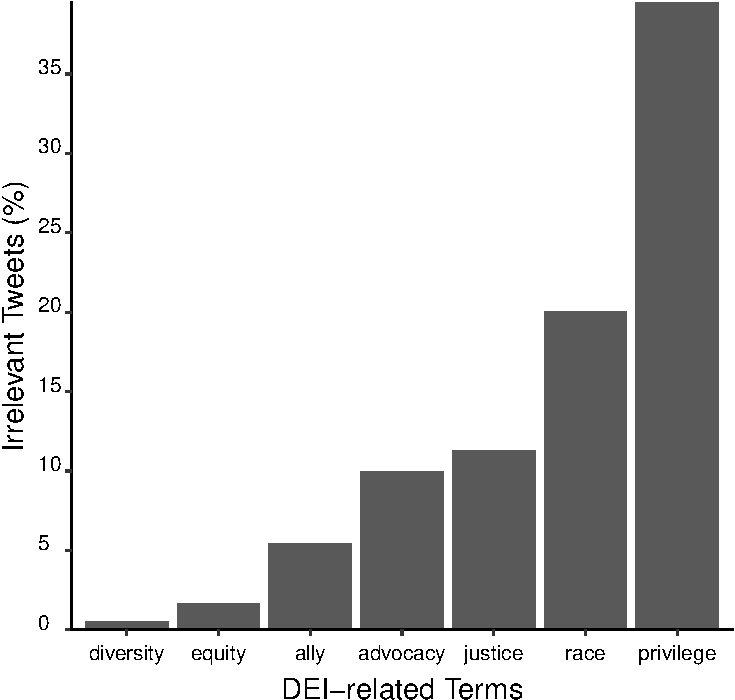
\includegraphics{Bruna_Supplement_files/figure-latex/FigS1-1} 

}

\caption{Percentage of irrelevant tweets atrtibuted to seven different DEI search terms. Note that this percentage is a conservative estimate, as it is based on a preliminary review.}\label{fig:FigS1}
\end{figure}

\begingroup\fontsize{12}{14}\selectfont

\begin{longtable}[l]{lccc}
\caption{\label{tab:Table1}Irrelevant tweets attributed to seven different DEI terms and the total number of tweets for each term in the original dataset. Note that this percentage is a conservative estimate, as it is based on a preliminary review.}\\
\toprule
DEI Term & Irrelevant Tweets (N) & Total Tweets (N) & \% Irrelevant\\
\midrule
diversity & 174 & 31268 & 0.56\\
equity & 270 & 16374 & 1.65\\
ally & 377 & 6953 & 5.42\\
advocacy & 512 & 5128 & 9.98\\
justice & 2491 & 22090 & 11.28\\
race & 5051 & 25167 & 20.07\\
privilege & 1382 & 3498 & 39.51\\
\bottomrule
\end{longtable}
\endgroup{}

\begingroup\fontsize{12}{14}\selectfont

\begin{longtable}[l]{ll}
\caption{\label{tab:Table2}Sample tweets incorrectly attributed to different DEI terms.}\\
\toprule
DEI Term & sample irrelevant tweet\\
\midrule
advocacy & a passionate physician and educator commited ot medical education pati\\
advocacy & the basic trial advocacy class at the uarizonalaw school argued their\\
advocacy & students in the basic trial advocacy class at the uarizonalaw had thei\\
ally & allymahoney11 y grades can be given for students if the faculty member\\
ally & allyrae12508 congratulations\\
ally & allyrae12508 welcome to the sun devil family\\
diversity & a new university of arizonaled study uses big data to assess why the d\\
diversity & a new study coauthored by university of arizona researchers provides t\\
diversity & new uarizona research finds that sexual reproduction and multicellular\\
equity & judge rakoffs decision has the potential of really blowing up said bri\\
equity & highly speculative prof renee jones talks to businessinsider about pri\\
equity & rt hnbayld congrats alex mancebo jonesday boston office focuses his pr\\
justice & arizonapbs will honor the legacy of supreme court justice sandra day o\\
justice & asucrimjustice researchers have found that there is a higher likelihoo\\
justice & two weeks before her first year at asu carson swisher changed her majo\\
privilege & rt azathletics 90 years ago today beardown was born it is a privilege\\
privilege & rt uapolicechief thank u asuatoday amp uaaa for this very special hono\\
privilege & rt wendelldneal two of the greatest guys i have ever had the privilege\\
race & join the beantowncats for the jeff coombs memorial virtual road race a\\
race & ronald a wilson ua title ix director and a former presiding judge for\\
race & join the beantowncats in the jeff coombs memorial road race on sept 9\\
\bottomrule
\end{longtable}
\endgroup{}


\clearpage
\renewcommand{\listfigurename}{Figure captions}


\end{document}
